\chapter{Errors in Dataset Similarity in Datasets and Images}
Step 2 og our scheme




\section{Labelling errors}
\noindent Labels are crucial because they serve as the foundation for training and evaluating machine learning models, particularly in supervised learning
\begin{itemize}
    \item Ground truth: the labels that the AI model should learn to predict or approximate
\end{itemize}

\subsubsection{Labels in databases for AI}
\begin{itemize}
    \item Model training: key in semi and supervised learning
\end{itemize}
\begin{figure}[H]
    \centering
    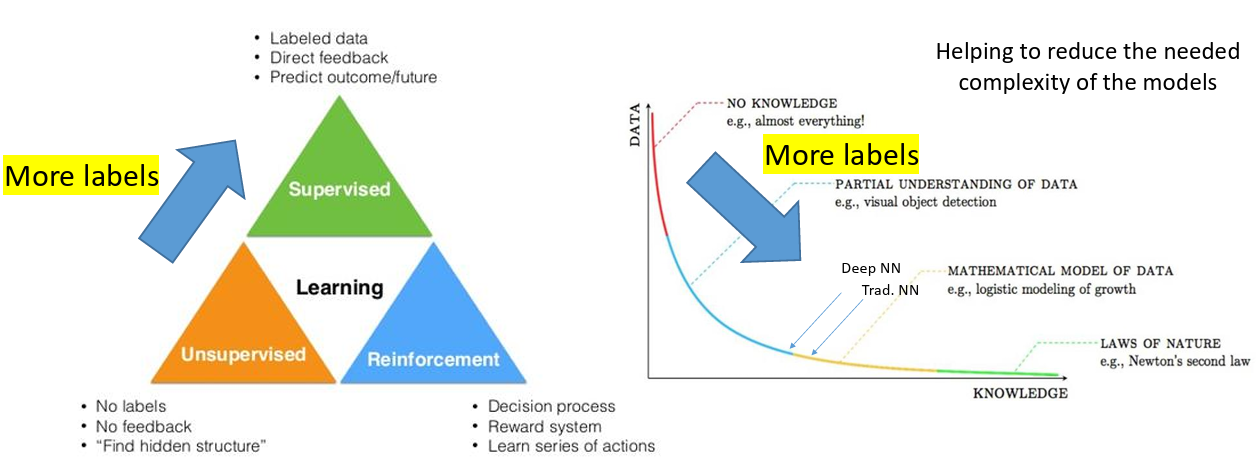
\includegraphics[width=0.8\linewidth]{09-10/images/labels.png}
\end{figure}

\begin{itemize}
    \item \textbf{Evaluation/Validation:} to assess the performance of a single trained AI model
    \item \textbf{Benchmarking/Ranking:} different models From labels you can process figures of merits (e.g., accuracy). Labeled datasets are commonly used as benchmarks for comparing the performance of different AI models, algorithms, or approaches
    \item \textbf{Model interpretability:} labels can also help explain the AI model's decisions, making it more transparent and interpretable (Supervised dataset helps explainability).
    \item \textbf{Transfer learning:}  Labeled data from one domain or task can be used to pre-train models for other related tasks or domains saving time and resources, specially when labeled data is scarce for the target domain (Adding specific images according the labels which are present)
\end{itemize}

\subsubsection{Label Errors in Dataset}
\noindent Some examples of labeling errors are from the previous lessons
\begin{itemize}
    \item Sample is correct, but the label is wrong (it's a dog but AI says it's a cat)
    \item The sample is misleading or incomplete (Data Leakage)
\end{itemize}

\noindent \textbf{Human supervisors are the typical sources of labels for our datasets}
\begin{itemize}
    \item Direct supervisor errors
    \item Data interchange/automatic conversion errors (un bodybuilder non è grasso)
\end{itemize}

\subsubsection{Basic checks for labelling errors}
\begin{itemize}
    \item Same input vectors 
    \begin{itemize}
        \item With same labels 
        \item With opposite labels (training problems!)
    \end{itemize}
    \item What to check in the training and validation database even it is not easy with large DB 
\end{itemize}

\subsubsection{Basic checks for duplications: hash functions}
\noindent If you are dealing with large data/vectors a simple comparison if xi is equal to xj requires element2element or pixel2pixel 

\noindent The comparison is time comsuming
\begin{itemize}
    \item Using a standard file \textit{hash} (if already available)
    \item Create \textit{image-hash} information offline (Specific hash functions for images are available)
\end{itemize}

\subsubsection{Basic checks for duplications/similarity}
\noindent Even if you are dealing with images or vectors (or unstructured data) is NOT just about if xi is equal to xj but something like if \textit{similarity} of xi and xj > of a fixed threshold


\section{Similarity }

\subsubsection{Why performing checks for similarity}
\begin{itemize}
    \item Too similar data/images are providing little more information
    \item Make the dataset more complex to be handled
    \item The similarity metrics must be tuned according to your application
\end{itemize}

\noindent Too much similarity is a waste of space and time but data Augmentation improve generalization 

\subsection{Similarity in datasets}




\subsection{in images}

\section{Main points}